\documentclass[12pt]{article}
\usepackage[utf8]{inputenc}
\usepackage{float}
\usepackage{amsmath}


\usepackage[hmargin=3cm,vmargin=6.0cm]{geometry}
%\topmargin=0cm
\topmargin=-2cm
\addtolength{\textheight}{6.5cm}
\addtolength{\textwidth}{2.0cm}
%\setlength{\leftmargin}{-5cm}
\setlength{\oddsidemargin}{0.0cm}
\setlength{\evensidemargin}{0.0cm}

%misc libraries goes here
\usepackage{tikz}
\usepackage{tabularx}

\begin{document}

\section*{Student Information } 
%Write your full name and id number between the colon and newline
%Put one empty space character after colon and before newline
Full Name :  Mert Kaan YILMAZ\\
Id Number :  2381093\\

% Write your answers below the section tags
\section*{Answer 1}
\textbf{a)} \\ 
    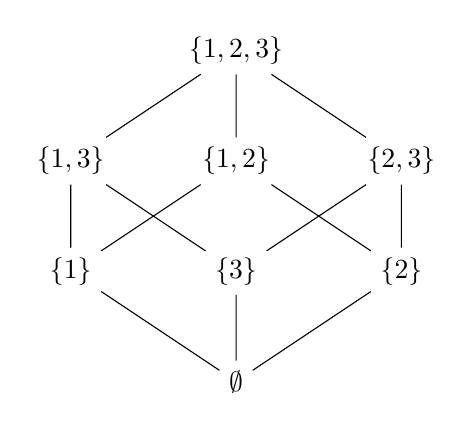
\begin{tikzpicture}[scale=.7]
      \node (123) at (0,3) {$\{1,2,3\}$};
      \node (23) at (3,1) {$\{2,3\}$};
      \node (12) at (0,1) {$\{1,2\}$};
      \node (13) at (-3,1) {$\{1,3\}$};
      \node (2) at (3,-1) {$\{2\}$};
      \node (3) at (0,-1) {$\{3\}$};
      \node (1) at (-3,-1) {$\{1\}$};
      \node (empty) at (0,-3) {$\emptyset$};
      \draw (empty) -- (1) -- (13) -- (123) -- (12) -- (1);
      \draw (empty) -- (2) -- (23) -- (123);
      \draw (12) -- (2);
      \draw (empty) -- (3) -- (13);
      \draw (3) -- (23);
    \end{tikzpicture} \\
\textbf{b)} The poset consisting of all the subsets of \{1,2,3\} is a lattice, because for every pair of objects exist, there is unique greatest lower bound and least lower bound. \\
The greatest lower bound of two subsets is the intersection of the two subsets \\such that $\{1,2\}\cap\{2,3\} = \{2\}$ \\
The least upper bound of two subsets is the union of the two subsets \\such that $\{1,2\}\cup\{2,3\} = \{1,2,3\}$ \\
\textbf{c)} $\{1,2,3\}$ is the maximal element. \\
\textbf{d)} $\emptyset$ is the minimal element. \\ 
\textbf{e)} Yes. $\{1,2,3\}$ is the greatest element. \\
\textbf{f)} Yes. $\emptyset$ is the least element. \\ 
\textbf{g)} Least upper bound of $\{1\}$ and $\{3\}$ is $\{1,3\}$.\\



\section*{Answer 2}
\textbf{a)} deg(a)+deg(b)+deg(c)+deg(d)+deg(e) = 2+4+2+3+3 = 14\\
\textbf{b)} If there is an edge between two nodes such that an edge e between x and y, row x column y and row y column x od adjacency matrix will be 1. Therefore, number\_of\_edges x 2 is our answer $\rightarrow$ 7x2 = 14\\
\textbf{c)} The number of one's is equals to sum of vertex degrees on the graph. Therefore the answer is deg(a)+deg(b)+deg(c)+deg(d)+deg(e) = 14 \\
\newpage
\textbf{d)} Yes it has a complete graph with at least three vertices as a subgraph.\\
For example: \\
\begin{figure}[H]
    \centering
	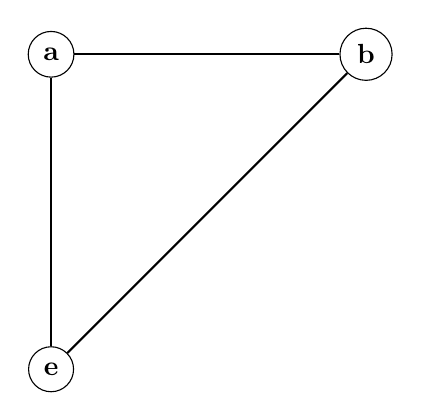
\begin{tikzpicture}
	
	\node[shape=circle,draw=black] (a) at (0, 4)     {\textbf{a}};
	\node[shape=circle,draw=black] (b) at (4, 4)     {\textbf{b}};
	\node[shape=circle,draw=black] (e) at (0, 0)     {\textbf{e}};
	
	\path[-, thick] (a) edge (b);
	\path[-, thick] (a) edge (e);
	\path[-, thick] (b) edge (e);
	
	\end{tikzpicture} 
	\caption{A complete graph as a subgraph with with at least three vertices.}	
	\label{fig:d}
\end{figure}
\textbf{e)} It's not a bipartite graph. To make one, we can remove vertex a and d. \\
    \begin{figure}[H]
    	\centering
    	\begin{tikzpicture}
    	
    	\node[shape=circle,draw=black] (b) at (4, 4)     {\textbf{b}};
    	\node[shape=circle,draw=black] (c) at (6, 2)     {\textbf{c}};
    	\node[shape=circle,draw=black] (e) at (0, 0)     {\textbf{e}};
    	
    	\path[-, thick] (b) edge (c);
    	\path[-, thick] (b) edge (e);
    
    	
    	\end{tikzpicture} 
    	\caption{After removing vertex a and d.}	
    	\label{fig:e}
    \end{figure}
\textbf{f)} For all edges, there are two alternatives in terms of direction. Therefore, our answer is $2^7 = 128$ \\
\textbf{g)} The length of the simple longest path in G is 7.\\
We can write this path as: e-a-b-e-d-b-c-d \\
\textbf{h)} The graph G has only one connected component, since we can reach all other vertices by choosing any vertex on the graph.\\
\textbf{i)} There is no Euler circuit, because in the graph, there are two vertices whose degrees are odd.\\
\textbf{j)} Yes it has Euler a path such that e-a-b-e-d-c-b-d. \\
\textbf{k)} Yes it has a Hamilton circuit such that a-e-d-c-b-a. \\
\textbf{l)} Yes it has a Hamilton path. For example: a-e-d-b-c. \\

\section*{Answer 3}
The graphical arrangement, namely the position of vertices and angle of edges make them different, but they are the same graph. \\
The number of vertices of G and H respectively: 8 and 8 \\
The number of edges of G and H respectively: 16 and 16 \\
Each vertices on G and H have degree of 4. \\
Also, Let t be a bijective function from G to H. Let the correspondence between graphs be: \\
t(a) = a', t(b) = c', t(c) = e', t(d) = g', t(e) = b', t(f) = h',  t(g) = d', t(h) = f', \\

Since above equalities hold and and above correspondence shows that the adjacency is preserved for all vertices, G and H graphs are isomorphic.
\section*{Answer 4}
I will use the notation {A,b} (in the table) for this question where A denotes the shortest path until the current node, and b denotes the path length. \\
\textbf{Step 1:} First we assign all node distances as infinity for all nodes except starting node a, which is clearly 0. (Because it's starting node.) \\
\textbf{Step 2:} The next vertex is b since it has minimum distance 3. We update the values of c and f. \\
\textbf{Step 3:} The next one is h. We update f and i. \\
\textbf{Step 4:} We randomly choose e, and there is no update. \\
\textbf{Step 5:} Choose c, update d, g, and f. \\
\textbf{Step 6:} The next on is i. Update j. \\
\textbf{Step 7:} We again randomly choose f, update j. \\
\textbf{Step 8:} Choose d, and update k. \\
\textbf{Step 9:} Randomly choose k, There is no update. \\
\textbf{Step 10:} Choose j, There is no update. \\
\textbf{Step 11:} Choose g, There is no update. \\


\begin{center}
\begin{tabular}{ | m{5em} | m{10cm}| m{2.5cm} | } 
  \hline
        \textbf{Node} & \textbf{Change} & \textbf{Final} \\
        \hline
            a  & \{$\emptyset,\infty$\}$\rightarrow$\{$\emptyset$,0\}  & \{$\emptyset$,0\}  \\
        \hline
            b  & \{$\emptyset,\infty$\}$\rightarrow$\{a,3\}  & \{a,3\}  \\
        \hline
            c  & \{$\emptyset,\infty$\}$\rightarrow$\{a-b,5\}  & \{a-b,5\}  \\
        \hline
            d  & \{$\emptyset,\infty$\}$\rightarrow$\{a-b-c,8\}  & \{a-b-c,8\}  \\
        \hline
            e  & \{$\emptyset,\infty$\}$\rightarrow$\{a,5\}  & \{a,5\}  \\
        \hline
            f  & \{$\emptyset,\infty$\}$\rightarrow$\{a-b,10\}$\rightarrow$\{a-h,9\}$\rightarrow$\{a-b-c,7\}  & \{a-b-c,7\}  \\
        \hline
            g  & \{$\emptyset,\infty$\}$\rightarrow$\{a-b-c,11\}  & \{a-b-c,11\}  \\
        \hline
            h  & \{$\emptyset,\infty$\}$\rightarrow$\{a,4\}  & \{a,4\}  \\
        \hline
            i  & \{$\emptyset,\infty$\}$\rightarrow$\{a-h,6\}  & \{a-h,6\}  \\
        \hline
            j  & \{$\emptyset,\infty$\}$\rightarrow$\{a-h-i,12\}$\rightarrow$\{a-b-c-f,10\}  & \{a-b-c-f,10\}  \\
        \hline
            k  & \{$\emptyset,\infty$\}$\rightarrow$\{a-b-c-d,10\}  & \{a-b-c-d,10\}  \\
        \hline
\end{tabular}
\end{center}
Therefore shortest path from a to j is a-b-c-f-j with cost 10.

\newpage
\section*{Answer 5}
\textbf{a)} For Kruskal’s minimum spanning tree algorithm, sort all the edges in non-decreasing order of their weight. \\
(a-b), (e,c), (c-f), (e-f), (a-d), (b-c), (b-e), (d-e), (a-e) \\
Pick the smallest edge and if it's not form a cycle, add it to the tree. The order is: \\
(a-b), (e,c), (c,f), (a,d), (b,c) \\
\textbf{b)} \\
    \begin{figure}[H]
    	\centering
    	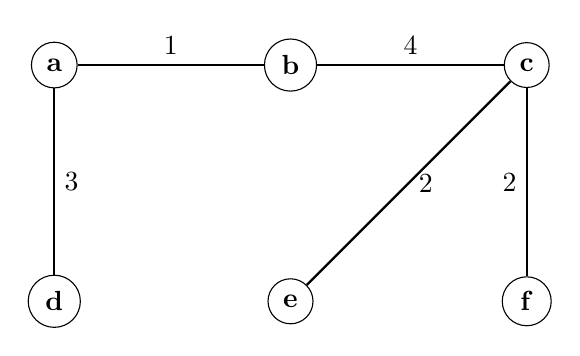
\begin{tikzpicture}
    	
    	\node[shape=circle,draw=black] (a) at (0, 3)     {\textbf{a}};
    	\node[shape=circle,draw=black] (b) at (3, 3)     {\textbf{b}};
    	\node[shape=circle,draw=black] (c) at (6, 3)     {\textbf{c}};
    	\node[shape=circle,draw=black] (d) at (0, 0)     {\textbf{d}};
    	\node[shape=circle,draw=black] (e) at (3, 0)     {\textbf{e}};
    	\node[shape=circle,draw=black] (f) at (6, 0)     {\textbf{f}};
    	
    	\path[-, thick] (a) edge node[above]{1} (b);
    	\path[-, thick] (b) edge node[above]{4} (c);
    	\path[-, thick] (a) edge node[right]{3} (d);
    	\path[-, thick] (c) edge node[right]{2} (e);
    	\path[-, thick] (c) edge node[left]{2} (f);
    	
    	\end{tikzpicture} 
    	\caption{Minimum spanning tree of graph G.}	
    	\label{fig:g5}
    \end{figure}
\textbf{c)} No, it's not. Since there are three edges with same weight 2, there are more than one minimum spanning tree. Therefore, minimum spanning tree is not unique.\\

\section*{Answer 6}
\textbf{a)} \\
The number of vertices: 13\\
The number of edges: 12\\
The height of T: 4\\\\
\textbf{b)} w-s-m-t-q-x-n-y-u-z-v-r-p\\\\
\textbf{c)} s-w-q-m-t-p-x-u-n-y-r-v-z\\\\
\textbf{d)} p-q-s-w-t-m-r-u-x-y-n-v-z\\\\
\textbf{e)} It's not a full binary tree, because a full binary tree has nodes which have exactly zero or two nodes. S, t, y, and v vertices have only one child. Therefore it's not a full binary tree.\\

\end{document}
